\documentclass[12pt]{book}

\usepackage{amsmath}
\usepackage{amssymb}
\usepackage{graphicx}
\usepackage[hidelinks]{hyperref}
\usepackage{bm}
\usepackage{dcolumn}
\usepackage{multirow}
\usepackage{listings}
\usepackage{authblk}
\usepackage{rotating}

\graphicspath{{../images/}}
\DeclareGraphicsExtensions{.eps,.png,.pdf}
\DeclareMathOperator{\sech}{sech}
\newcolumntype{d}[1]{D{.}{.}{#1} }
\lstset{
	basicstyle=\tiny\ttfamily,
	frame=single,
	columns=fixed,
	breaklines=true
}

\renewcommand{\figurename}{Figure}
\newcommand{\figurenames}{Figures}
%\newcommand{\figname}{Figure}
%\newcommand{\fignames}{Figures}
\newcommand{\figname}{Fig.}
\newcommand{\fignames}{Figs.}
\newcommand{\equationname}{Equation}
\newcommand{\equationnames}{Equations}
%\newcommand{\eqnname}{Equation}
%\newcommand{\eqnnames}{Equations}
\newcommand{\eqnname}{Eq.}
\newcommand{\eqnnames}{Eqs.}

\providecommand{\HUGE}{\Huge}
\newlength{\drop}
\newcommand*{\titleGM}{\begingroup
\drop = 0.1\textheight
%\vspace*{\baselineskip}
\vfill
  \hbox{%
  \hspace*{0.2\textwidth}%
  \rule{1pt}{\textheight}
  \hspace*{0.05\textwidth}%
  \parbox[b]{0.75\textwidth}{
  \vbox{%
    \vspace{\drop}
    {\noindent\HUGE\bfseries Sonar Workbench\\[0.5\baselineskip]
               v3.2}\\[2\baselineskip]
    {\Large\itshape User's Guide}\\[4\baselineskip]
    {\Large Thomas J Deal, MSc, PhD}\par
    \vspace{0.5\textheight}
    {\noindent Naval Undersea Warfare Center, Newport, RI}\\[\baselineskip]
    }% end of vbox
    }% end of parbox
  }% end of hbox
\vfill
\null
\endgroup}

\begin{document}

\pagestyle{empty}
\titleGM
\cleardoublepage

\frontmatter
\pagestyle{headings}

\tableofcontents
\listoftables
\listoffigures

\chapter{Abstract}
Sonar Workbench is a suite of Matlab tools for the design and analysis of sonar systems. Version 1.0 focused on array construction and beam pattern construction and analysis. Version 2.0 added TEAMS interface support. Version 3.0 vectorized position and orientation parameters for increased efficiency. Version 3.1 added full support for calculating beam patterns in the body frame for rotated arrays. Version 3.2 removed Signal Processing Toolbox dependencies and added 2D beam pattern analysis tools. Sonar Workbench includes multiple element types, from which the user constructs an array with arbitrary element position and orientation. The user defines complex weights for each element to create a beam with the desired shape, which can be evaluated at any elevation and azimuthal angles, plotted in 3D space, and measured for beam width and directivity index.

\cleardoublepage

\mainmatter

\chapter{Introduction}\label{ch:intro}

Sonar Workbench is a suite of Matlab tools for the design and analysis of sonar systems. Sonar Workbench includes multiple element types, from which the user constructs an array with arbitrary element position and orientation. The user defines complex weights for each element to create a beam with the desired shape, which can be evaluated at any elevation and azimuthal angles, plotted in 2D or 3D space, and measured for beam width and directivity index.

This user's guide is intended to introduce a new user to Sonar Workbench, the array theory it implements, and its usage in the Matlab environment. Much of the content is adapted from \emph{An Introduction to Sonar Systems Engineering} \cite{Ziomek}, which is recommended as a companion resource for the user interested in understanding more of the theory. Chapter~\ref{ch:coord} introduces the coordinate system and reference frames used in Sonar Workbench. Chapter~\ref{ch:element} explains how to define elements and lists the built-in element types. Chapter~\ref{ch:array} describes the process to build arrays consisting of uniform or mixed element types. Chapter~\ref{ch:beam} defines beams and demonstrates a method for calculating amplitude and phase weights for conventional beamforming. Chapter~\ref{ch:analysis} demonstrates how Sonar Workbench implements these concepts and conventions and shows the user how to use it for their own analysis.

The example element, array, and beam definitions used in this guide can be found in the \texttt{test} folder, along with a script \texttt{CreateSampleBeam.m} the user can execute to demonstrate the features of Sonar Workbench. 

\section*{Revision History}

\begin{description}
\item[v1.0] Initial capability for array construction and beam pattern construction and analysis. 
\item[v2.0] Added TEAMS interface support. 
\item[v3.0] Vectorized position and orientation parameters for increased efficiency. 
\item[v3.1] Added full support for calculating beam patterns in the body frame for rotated arrays. 
\item[v3.2] Removed Signal Processing Toolbox dependencies and added 2D beam pattern analysis tools. 
\item[v3.3] Added plotting for omnidirectional and cosine element shapes.
\item[v3.4] Removed inputparser() code for codegen and Simulink compatibility.
\end{description}
\section{Coordinate System and Reference Frames}\label{sec:coord}
Sonar Workbench uses a right-handed, Cartesian coordinate system known as North-East-Down (NED), as shown in \figname~\ref{fig:NED}. In this coordinate system, the first coordinate, $x$, points north, the second coordinate, $y$, points east, and the third coordinate, $z$, points down. Roll, $\gamma$, is rotation about the $x$ axis, pitch, $\theta$, is rotation about the $y$ axis, and yaw, $\psi$, is rotation about the $z$ axis. The NED coordinate system is ideal for underwater applications, because depth is measured downward from the surface, yaw is measured clockwise from north, and pitch is measured relative to the horizontal plane.

\begin{figure}[!ht]
\begin{center}
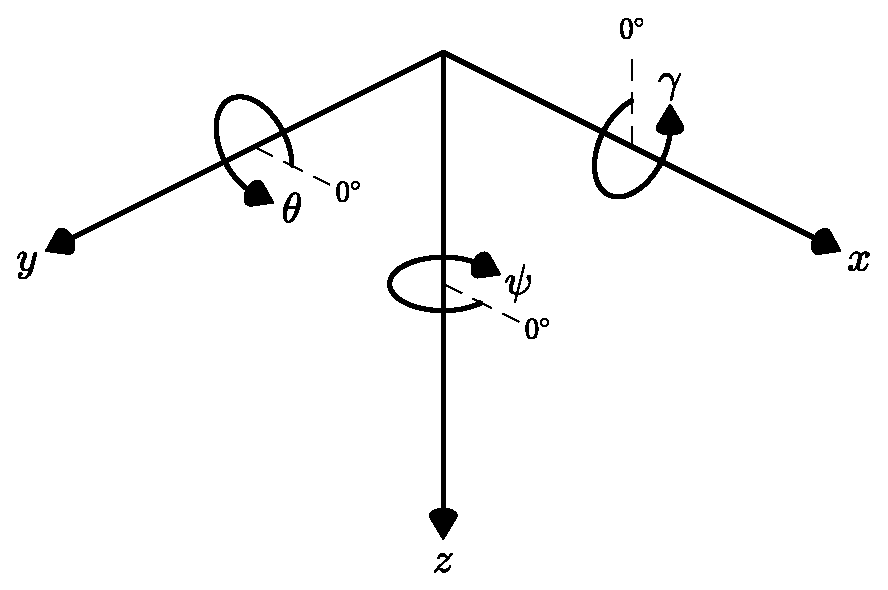
\includegraphics[width=3in]{NEDCoordinateSystem}
\caption{\label{fig:NED}NED coordinate system}
\end{center}
\end{figure}

Sonar Workbench uses three reference frames: the element frame, the array frame, and the body frame. All frames use the NED coordinate system, and each frame can be located relative to another by a combination of translations\footnote{displacement along the $x$, $y$, or $z$ axes} and rotations.

The element frame is always located at the center of the element, with the element's maximum response axis aligned with the $+x$ axis. Exceptions to this alignment are the omnidirectional element, which has no maximum response axis, and the linear element, which the user specifies as initially parallel to one of the three axes ($x$,$y$,$z$) in the element frame. For planar piston elements, the element face lies in the element frame $y$-$z$ plane.

Each element in an array can have arbitrary translation and rotation in the array frame. The array frame origin and orientation is entirely up to the user, but it is typical for planar arrays to be located in center of the array frame's $y$-$z$ plane and for volumetric arrays' geometric center to be located at the origin of the array frame.

The entire array can also be arbitrarily translated and rotated relative to the body frame. For example, a planar array on the nose of a torpedo might have a simple translation along the body frame $x$ axis, while a flank array might have translations along the body $x$ and $y$ axes plus a rotation $\psi$ about the body frame $z$ axis. \figurename~\ref{fig:ReferenceFrames} shows an example of element, array, and body frames for a conformal flank array.

\begin{figure}[!ht]
\begin{center}
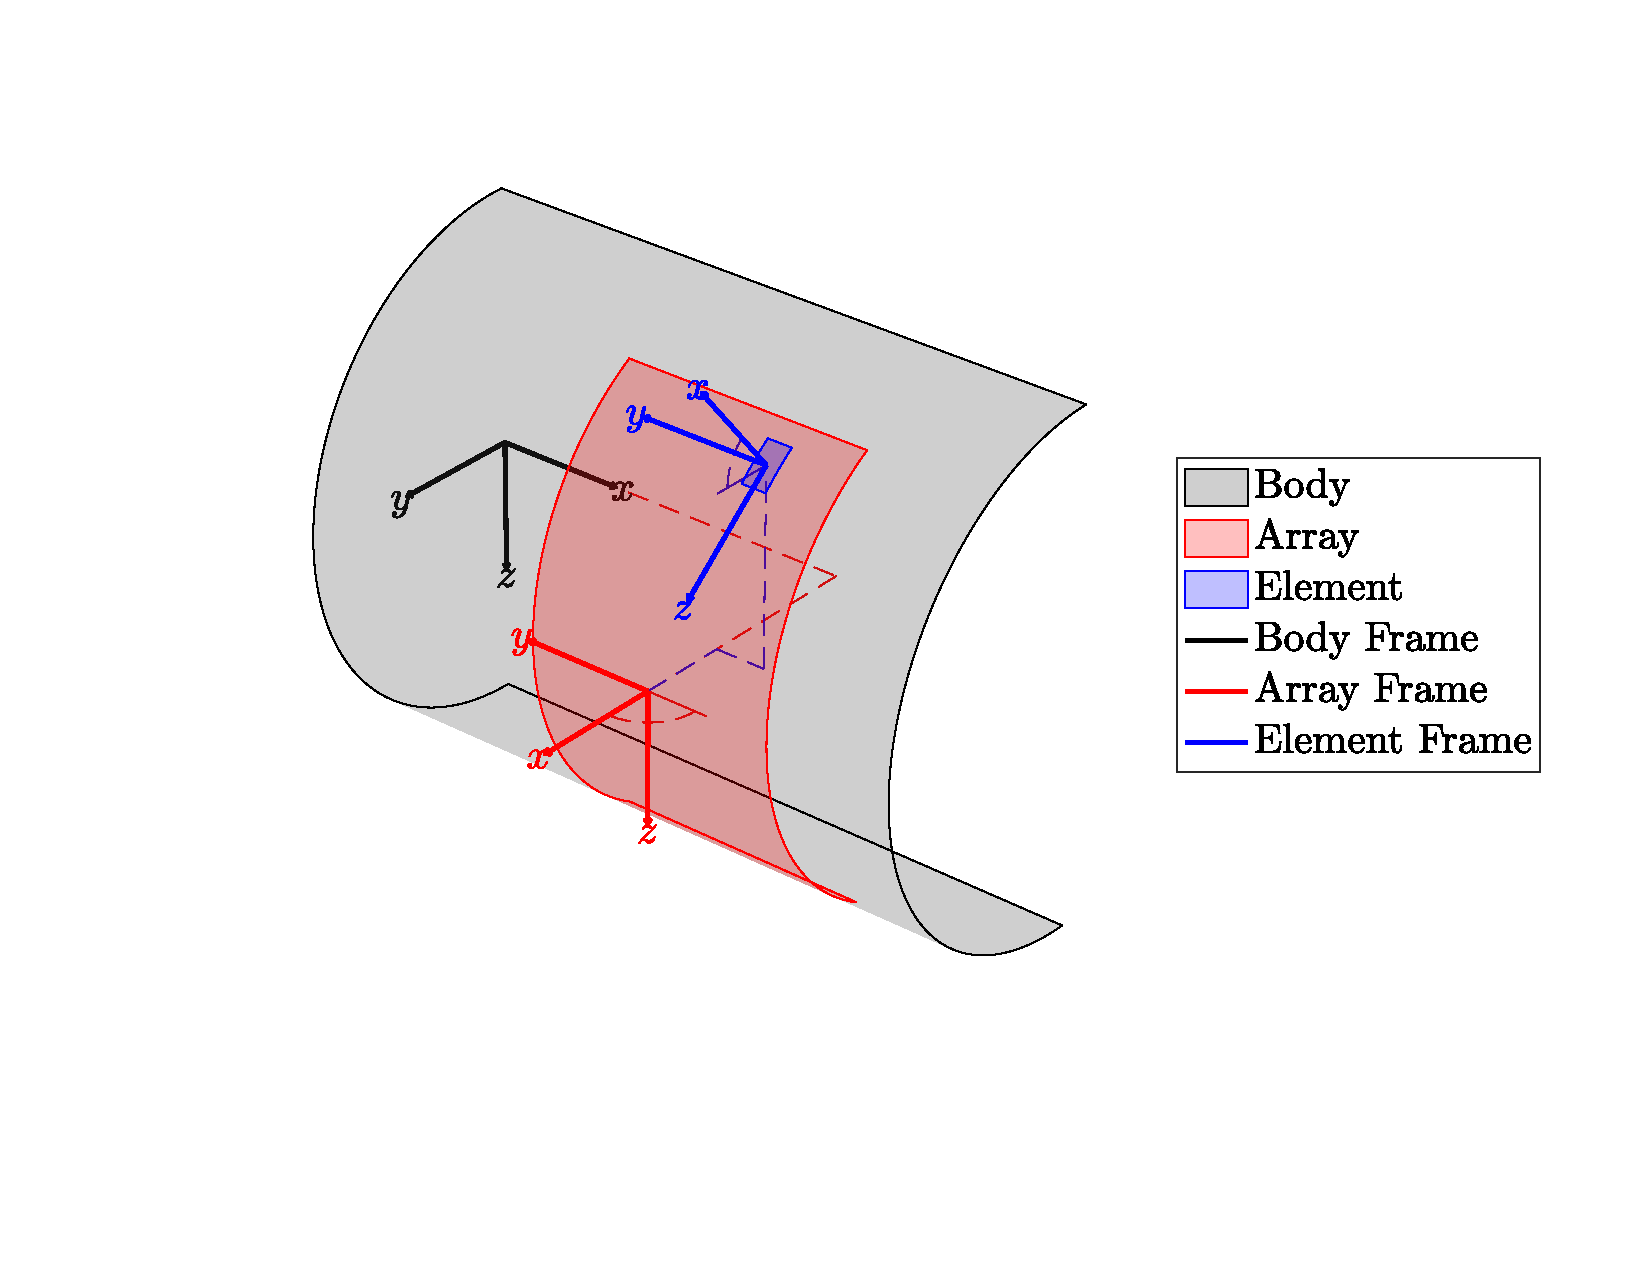
\includegraphics[width=\textwidth]{BodyArrayElementFrame}
\caption{\label{fig:ReferenceFrames}Body, array, and element frames for flank array example}
\end{center}
\end{figure}

Beam patterns are always computed in the body frame as a function of body azimuth angles $\psi$ and elevation angles $\theta$. Azimuth and elevation angles are measured from the body frame $+x$ axis. For simple analyses, the array and body frames can be aligned and colocated to produce beam patterns in the array frame. In this case, beam pattern angles $\psi$ and $\theta$ are measured from the array frame $+x$ axis. More details about element, array, and body frame alignments will be explained in Sections~\ref{sec:element} and \ref{sec:array}.

\section{Elements}\label{sec:element}

The transducer element is the fundamental building block for arrays and the starting point for analysis in Sonar Workbench. For the purpose of generating and analyzing beam patterns, specific electromechanical transduction methods do not need to be modeled; instead, the element's acoustic properties can be captured by modeling vibrations of the element's wetted surface. Hereafter, references to an element's geometry refer to the geometry of the element's wetted surface or face. Sonar Workbench treats each element as a uniformly vibrating surface, which is to say that it only models each surface's fundamental mode of vibration. Analyzing element response requires first, defining the element geometry, and second, evaluating that geometry at a specific acoustic wavelength to produce an element pattern.

\subsection{Element definition}

Sonar Workbench includes support for the element types listed in Table~\ref{tab:ElementTypes}. 

\begin{table}[!ht]
	\begin{center}
		\caption{Included element types}
		\label{tab:ElementTypes}
		\begin{tabular}{c|l} 
			\textbf{Element Type} & \textbf{Type String} \\
			\hline
			Omnidirectional  & \texttt{`OmnidirectionalElement'} \\
			Uniform Line & \texttt{`LinearElement'} \\
			Cosine & \texttt{`CosineElement'} \\
			Circular Piston & \texttt{`CircularPistonElement'} \\
			Rectangular Piston & \texttt{`RectangularPistonElement'} \\
			Annular Piston & \texttt{`AnnularPistonElement'} \\
			Hexagonal Piston & \texttt{`HexagonalPistonElement'} \\
		\end{tabular}
	\end{center}
\end{table}

An element structure holds the parameters that define the element geometry. The element structure must contain the \texttt{.type} field with a string corresponding to the name of a \texttt{.m} file that generates the corresponding element pattern. Table~\ref{tab:ElementTypes} lists the built-in element type strings, but the user can define additional element types by generating their own element pattern generator script with the same interface. 

The field \texttt{.baffle} dictates whether the element should be baffled by the element frame $y$-$z$ plane (e.g. arrays mounted to platforms) or unbaffled (e.g. towed arrays, sonobuoys). The omnidirectional, uniform line, and cosine elements can all be used with and without baffling. The piston elements' element patterns are all derived from equations assuming the piston is mounted in an infinite rigid baffle; therefore, it is recommended that the user set these element's \texttt{.baffle=1} for best results. Diffraction effects caused by finite baffle dimensions are beyond the scope of Sonar Workbench. 

For visualization purposes, fields \texttt{.shapex}, \texttt{.shapey}, and \texttt{shapez} contain vectors of element shape coordinates. The script \texttt{AddElementShape.m} generates these vectors for the element types listed in Table~\ref{tab:ElementTypes}. The other fields in the element structure depend on the element type, as listed in Table~\ref{tab:ElementFields}.

\begin{table}[!ht]
	\begin{center}
		\caption{Element structure fields}
		\label{tab:ElementFields}
		\begin{tabular}{c|c|l} 
			\textbf{Element Type} & \textbf{Field} & \textbf{Description} \\
			\hline
			\multirow{2}{*}{Uniform Line} & \texttt{.L} & length (m) \\
			& \texttt{.axis} & aligned axis \texttt{`x'}, \texttt{`y'}, \texttt{`z'} \\
			\hline
			Circular Piston & \texttt{.a} & radius (m) \\
			\hline
			\multirow{2}{*}{Rectangular Piston} & \texttt{.w} & width (m) \\
			& \texttt{.h} & height (m) \\
			\hline
			\multirow{2}{*}{Annular Piston} & \texttt{.a} & outer radius (m) \\
			& \texttt{.b} & inner radius (m) \\
			\hline
			Hexagonal Piston & \texttt{.a} & inscribed circle radius (m) \\	
		\end{tabular}
	\end{center}
\end{table}

Listing~\ref{lst:SampleElement} shows the contents of \texttt{SampleElement.m}, which defines a rectangular piston element.

\lstinputlisting[caption={\texttt{SampleElement.m}},label={lst:SampleElement}]{../../examples/SampleElement.m}

The user is free to add additional fields to the element structure for their own purposes. These will be ignored by Sonar Workbench.

\subsection{Element patterns}

Element geometry, coupled with an acoustic wavelength, defines the element pattern. The element pattern is the element's far-field directional response as a function of wavelength, azimuth and elevation, and it can be thought of as a spatial filter. Elements are assumed to be transducers, capable of transmitting and receiving sound, so there is no distinction between transmit and receive element patterns. 

Sonar Workbench uses the acoustic wavelength, $\lambda$, to calculate element patterns because it combines the frequency and sound speed into a single term. It is related to sound speed $c$, frequency $f$ in Hz or $\omega$ in rad/s, and wavenumber $k$ in m$^{-1}$ by
\begin{equation*}
\lambda = \frac{c}{f} = \frac{2\pi{c}}{\omega} = \frac{2\pi}{k}.
\end{equation*}

At its most general, the element pattern is the three-dimensional Fourier transform of the element's complex aperture function, $A(\lambda,x,y,z)$,
\begin{equation}
E(\lambda,\theta,\psi) = \int_{-\infty}^\infty\int_{-\infty}^\infty\int_{-\infty}^\infty A(\lambda,x,y,z)e^{j2\pi\left(\frac{\cos\theta\cos\psi}{\lambda}x + \frac{\cos\theta\sin\psi}{\lambda}y + \frac{\sin\theta}{\lambda}z\right)}dxdydz,\label{eq:VolumetricFT}
\end{equation}
For the piston elements, the element pattern reduces to a two-dimensional Fourier transform, since the element face lies in the $y$-$z$ plane,
\begin{equation}
E_{piston}(\lambda,\theta,\psi) = \int_{-\infty}^\infty\int_{-\infty}^\infty A(\lambda,y,z)e^{j2\pi\left(\frac{\cos\theta\sin\psi}{\lambda}y + \frac{\sin\theta}{\lambda}z\right)}dydz,\label{eq:PlanarFT}
\end{equation}
and for the uniform line array, it further reduces to a one-dimensional Fourier transform,
\begin{equation}
E_{line}(\lambda,\theta,\psi) = \int_{-\infty}^\infty A(\lambda,y)e^{j2\pi\frac{\cos\theta\sin\psi}{\lambda}y}dy,\label{eq:LinearFT}
\end{equation}
for a line array aligned with the $y$ axis. The finite element extents make the integration limits finite. For the simple elements included with Sonar Workbench, the assumption of uniform surface motion means that the aperture function is real-valued and equal to 1 over the entire element surface. This simplifies the integration for certain element geometries. These integrals have analytic solutions, which Sonar Workbench uses instead of evaluating the integrals numerically.

Element patterns are normalized such that they have unity gain along their maximum response axis. \figurename~\ref{fig:ElementPatterns} shows element patterns for each of the included element types listed in Table~\ref{tab:ElementTypes} for a wavelength equal to half of the element's maximum dimension. The uniform line element is aligned with the $y$ axis, and the cosine element is aligned with the $x$ axis. Note that the omnidirectional and cosine element patterns do not depend on wavelength.

\begin{sidewaysfigure}[!ht]
\begin{center}
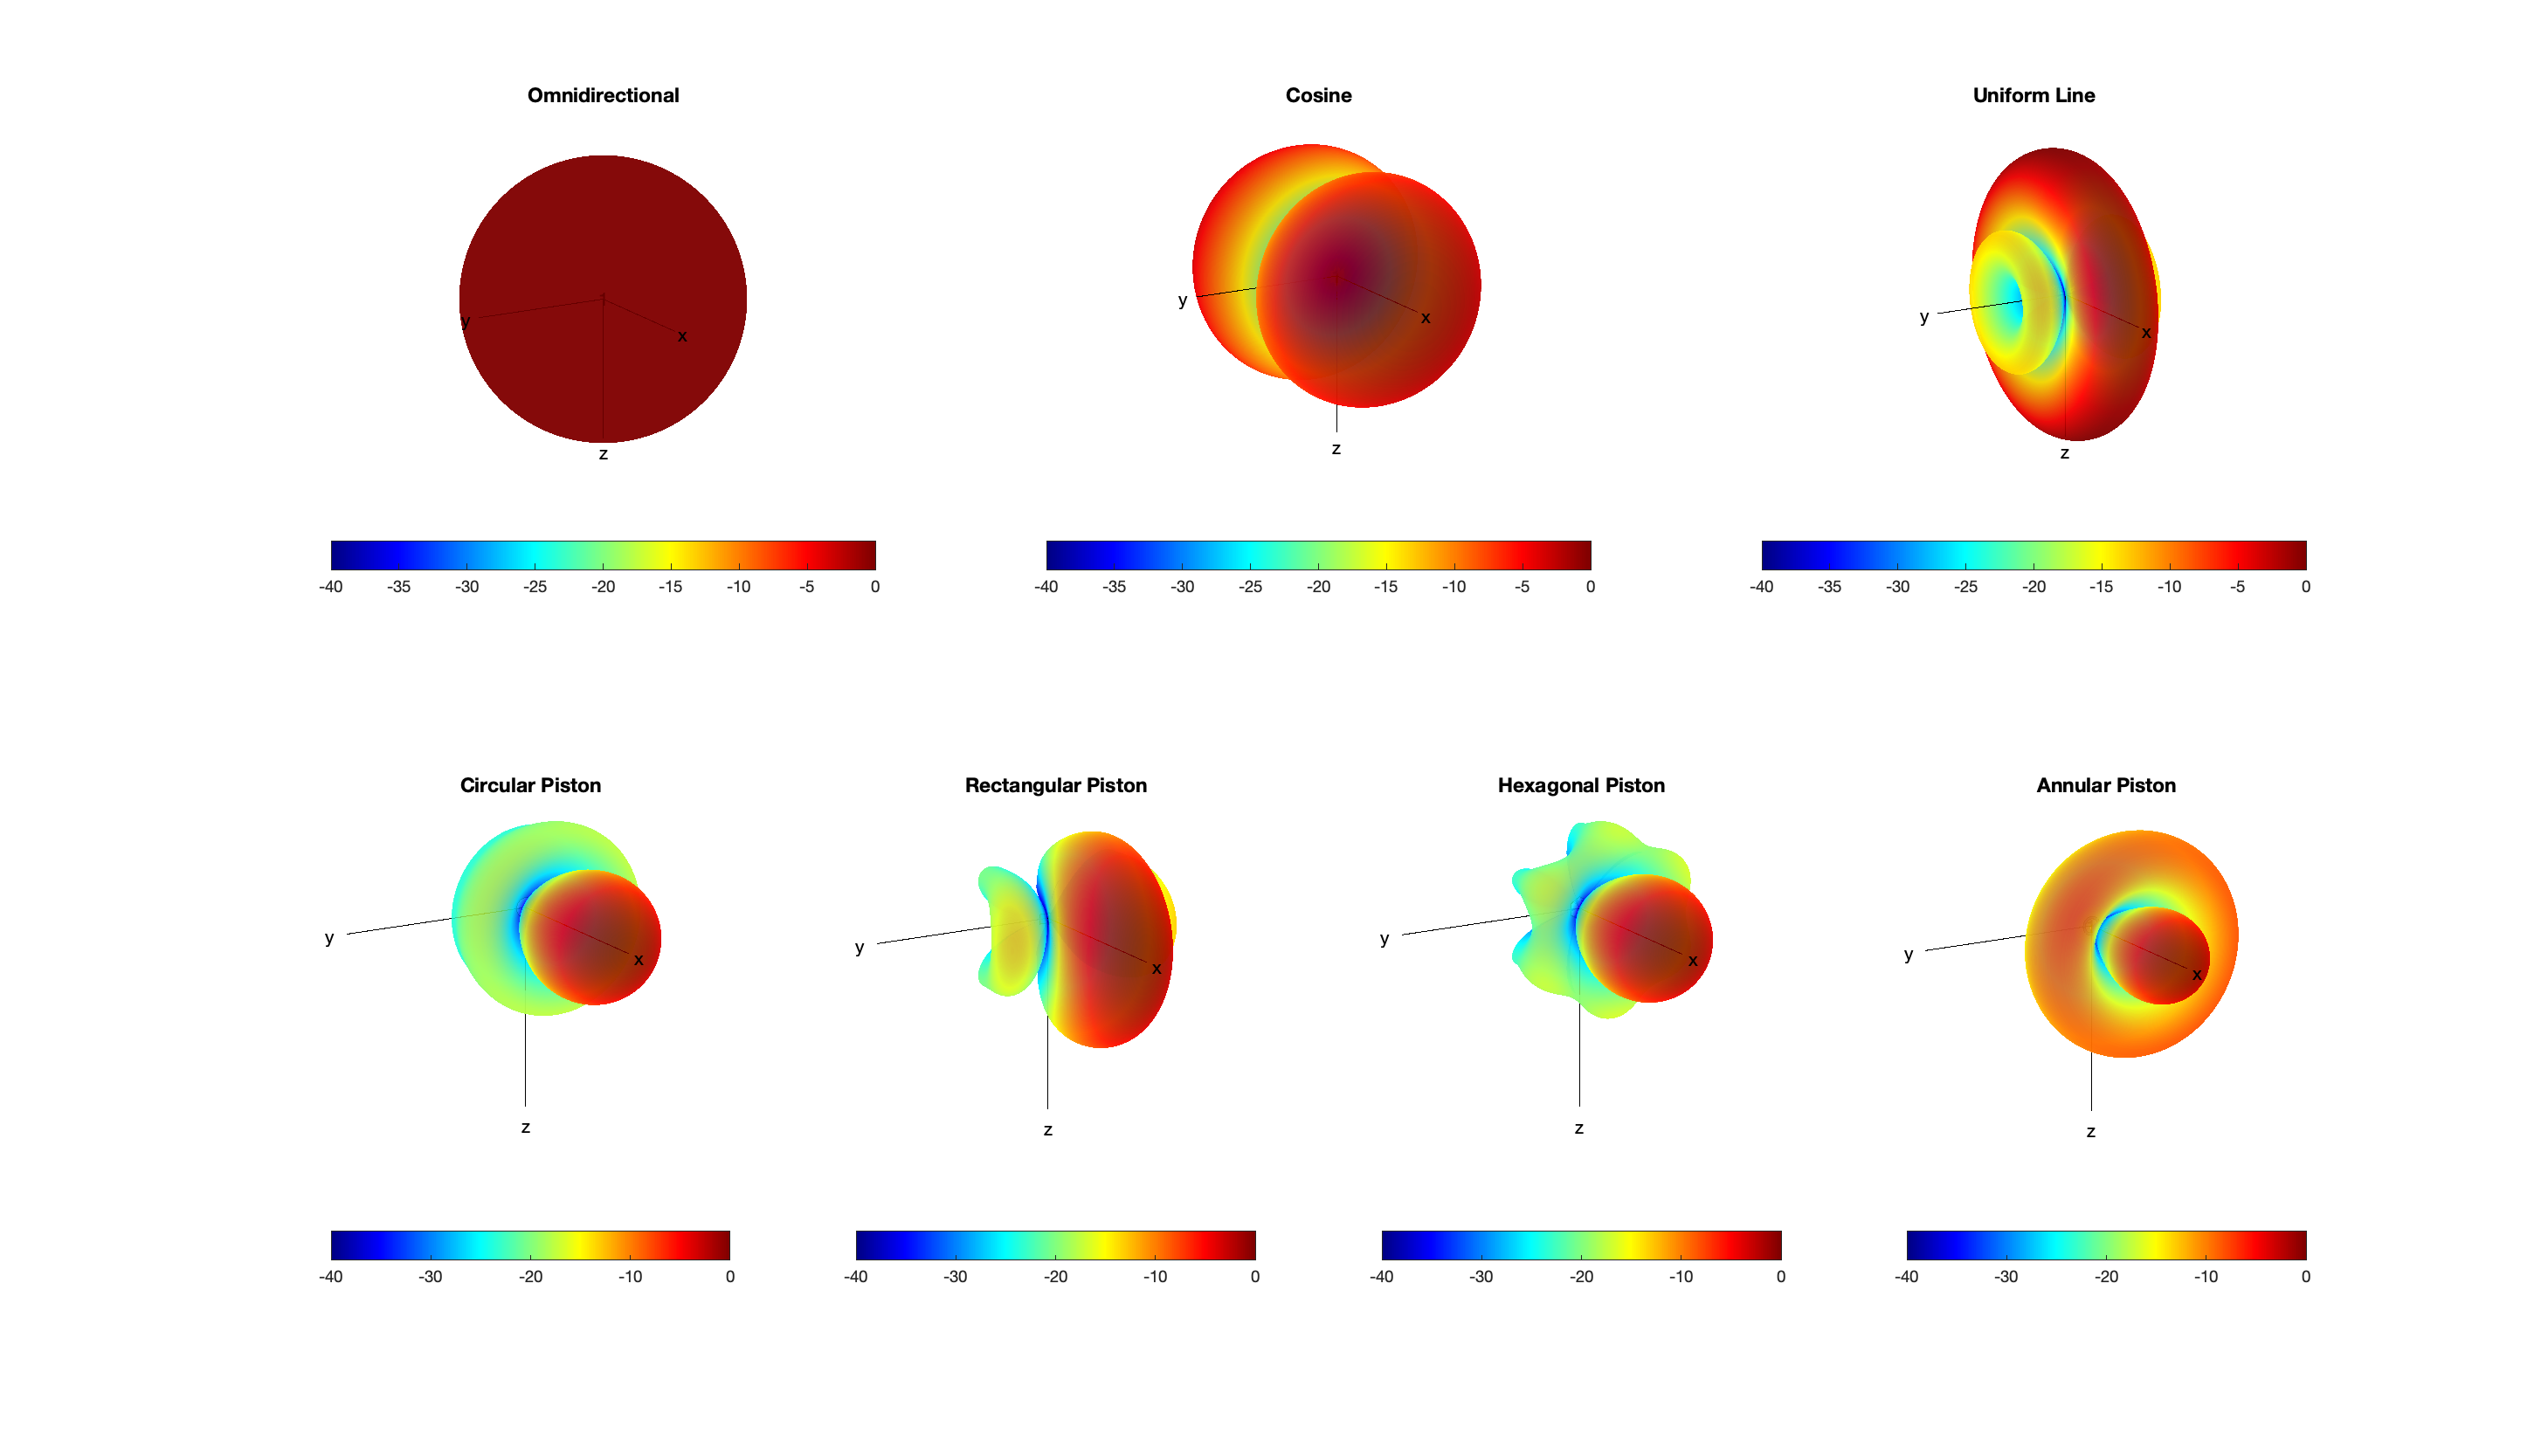
\includegraphics[width=8in]{ElementPatterns}
\caption{\label{fig:ElementPatterns}Element patterns for included element types (magnitude in dB)}
\end{center}
\end{sidewaysfigure}

\chapter{Arrays}\label{ch:array}

An array is a collection of elements. Each element in an array has a position and orientation in the array frame. The array itself also has a position and orientation in the body frame. Sonar Workbench supports arrays with mixed element types, e.g. vector sensor arrays with a mix of hydrophones (omnidirectional elements) and accelerometers (cosine elements). The array structure has fields which contain this information.

The field \texttt{.Ne} holds the integer number of elements in the array. The position, orientation, and element type fields are all column vectors of length \texttt{.Ne}. The user is free to choose any convenient element order, as long as that order is consistent across all fields. A (3$\times$\texttt{.Ne}) matrix determines the element positions in the array frame, \texttt{.ePos\_m}, with rows corresponding to $x$, $y$, and $z$, respectively, in units of meters. An additional (3$\times$\texttt{.Ne}) matrix determines the element orientations in the array frame, \texttt{.eOri\_deg}, with rows corresponding to roll, pitch, and yaw, in degrees. Array position and orientation are held in the (3$\times$1) vectors \texttt{.aPos\_m} and \texttt{.aOri\_deg}, respectively. Table~\ref{tab:ArrayFields} summarizes the fields in the array structure. 

\begin{table}[!ht]
	\begin{center}
		\caption{Array structure fields}
		\label{tab:ArrayFields}
		\begin{tabular}{c|l} 
			\textbf{Field} & \textbf{Description} \\
			\hline
			\texttt{.Ne} & number of elements \\
			\texttt{.Net} & number of unique element types \\
			\texttt{.Element} & vector of length \texttt{.Net} element structures \\
			\texttt{.ePos\_m} & element position matrix (m) \\
			\texttt{.eOri\_deg} & element orientation matrix ($^\circ$) \\
			\texttt{.eindex} & element type index (optional) \\
			\texttt{.aPos\_m} & array position vector (m) \\
			\texttt{.aOri\_deg} & array orientation vector ($^\circ$) \\
		\end{tabular}
	\end{center}
\end{table}

\section{Arrays with uniform element types}

When all the array elements are identical, the array structure does not need the \texttt{.eindex} field. An example array structure is found in \texttt{SampleArray.m}, shown in Listing~\ref{lst:SampleArray}.

\lstinputlisting[float,caption={\texttt{SampleArray.m}},label={lst:SampleArray}]{../../test/SampleArray.m}

This planar array contains 50 rectangular elements arranged in a grid 5 elements wide by 10 elements high. The geometry is shown in \figname~\ref{fig:SampleArray}, with elements numbered according to their order in the array structure.

\begin{figure}[!ht]
\begin{center}
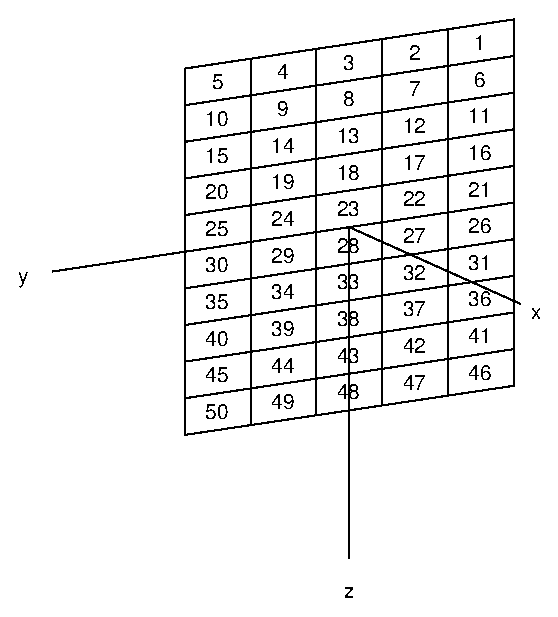
\includegraphics[width=3in]{SampleArray}
\caption{\label{fig:SampleArray}Example rectangular planar array}
\end{center}
\end{figure}

\clearpage
\section{Arrays with mixed element types}

For mixed-element arrays, the \texttt{.eindex} field must be a row vector of length \texttt{.Ne} integers. The user must first define an element structure array, with one entry for each unique element type. The \texttt{.eindex} field for each element must contain the 1-based index into the element structure array corresponding to its element type. The maximum value allowed is \texttt{.Net}.

An example is included in \texttt{SampleVSCardioid.m} for a simple vector sensor. The relevant portion is shown in Listing~\ref{lst:SampleVSCardioid}. This vector sensor consists of four elements: a hydrophone and three orthogonal accelerometers. The three accelerometers are identical except for their orientations, so there are a total of two unique elements. The hydrophone is \texttt{VS.Element(1)}, and the accelerometer is \texttt{VS.Element(2)}. The array structure is named \texttt{VS}, and the hydrophone is the first element, followed by the $x$, $y$, and $z$ accelerometers. This makes the first entry in \texttt{.eindex} equal to 1 and the rest of the entries equal to 2. Rows two and three of \texttt{.eOri\_deg} rotate elements 3 and 4 from the $x$ axis to the $y$ and $z$ axes, respectively.

\lstinputlisting[firstline=5,lastline=22,caption={\texttt{SampleVSCardioid.m}},label={lst:SampleVSCardioid}]{../../test/SampleVSCardioid.m}

\chapter{Beams}\label{ch:beam}

Once an array and element(s) have been defined, the user can generate any number of beam patterns by defining a set of wavelength-dependent, complex weights, $w(\lambda)$. Multiple beams can be calculated for the same array by changing these weights. The beam structure must contain these weights in a single field called \texttt{.ew}, which is a row vector of length \texttt{Array.Ne}.

In conventional (plane wave) beamforming, amplitude weights are used to adjust the width of the beam's main lobe and the magnitude of its sidelobes, and phase weights are used to steer the beam in azimuth and elevation. For a source in the array's acoustic near field, phase weights can also be used to focus the beam at a specified range. In adaptive beamforming, a complex set of weights is chosen to simultaneously maximize one criterion (e.g. signal level) and minimize one or more other criteria (e.g. noise level). Iterative methods that calculate complex weights to produce beams with prescribed main lobe dimensions and side lobe levels also exist.  Although the details of near-field focusing and adaptive beamforming are beyond the scope of this user's guide, Sonar Workbench can generate beam patterns for any complex weights the user derives.

\section{Conventional beamforming}

Conventional beamforming independently calculates amplitudes, $a_i$, and phases, $\phi_i$ to create complex weights $w_i=a_ie^{j\phi_i}$. Listing~\ref{lst:SampleBeam} shows an example of one beam that can be formed for the planar array example from Chapter~\ref{ch:array}. This example contains both amplitude and phase weights.

\lstinputlisting[caption={\texttt{SampleBeam.m}},label={lst:SampleBeam}]{../../test/SampleBeam.m}

\subsection{Amplitude weights}

Amplitude shading exploits the Fourier transform relationship between the beam's aperture function and its far field beam pattern. Consequently, sonar designers often use weights, or shading coefficients, taken from standard window functions. Examples include Uniform, Hanning, Hamming, and Chebyshev, as shown in \figname~\ref{fig:WindowFunctions}. The example beamformer uses two Chebyshev windows, one of length 5 in the horizontal direction, and one of length 10 in the vertical direction. The total weight for each element is the product of the two windows evaluated at its coordinate the horizontal and vertical direction.

\begin{figure}[!ht]
\begin{center}
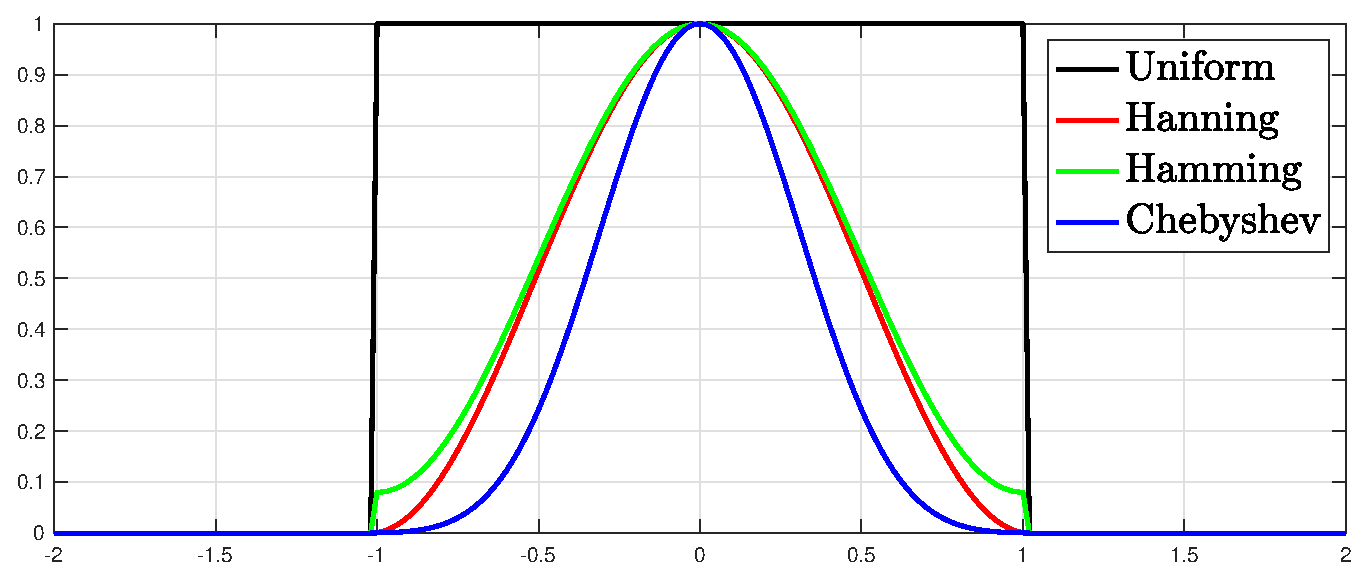
\includegraphics[width=\textwidth]{WindowFunctions}
\caption{\label{fig:WindowFunctions}Common window functions used for amplitude shading}
\end{center}
\end{figure}

Since the final beam pattern will be normalized for unity gain along its maximum response axis, the user is not required to normalize the amplitude weights or limit their amplitude. However, it is best to avoid negative amplitude weights and instead represent negative numbers with phase weights.

\subsection{Phase weights}

Without phase weights, i.e. the beam pattern weights are purely real, the beam pattern is unsteered. The user can steer the beam to an arbitrary elevation and azimuth, ($\theta_0$,$\psi_0$) using the following formula for the $i^{th}$ element's phase,
\begin{equation}
\phi_i(\lambda,\theta_0,\psi_0) = -2\pi\left(\frac{\cos\theta_0\cos\psi_0}{\lambda}x_i + \frac{\cos\theta_0\sin\psi_0}{\lambda}y_i + \frac{-\sin\theta_0}{\lambda}z_i \right).\label{eq:phasesteer}
\end{equation}
Note that the negative sign in the third term in \eqnname~(\ref{eq:phasesteer}) accounts for the definition of positive elevation angles in the negative $z$ direction, as shown in \figname~\ref{fig:NED}.
\chapter{Analysis}\label{ch:analysis}

Sonar Workbench includes built-in functions to assist with analysis.  Versions 1.0-3.0 concentrated on array building, conventional beam pattern synthesis, and beam pattern analysis.  Planned upgrades include support for adaptive beamforming, element and array radiation impedance, and array gain in anisotropic noise.

\section{Plotting arrays}

The function \texttt{PlotArray.m} creates a 3D plot of an array. Usage instructions are shown in Listing~\ref{lst:PlotArray}. The user must pass the array structure as the first parameter to \texttt{PlotArray.m}. This will produce a physical plot of the array, as shown in \figname~\ref{fig:SampleArray}. There are three optional inputs to \texttt{PlotArray.m}. The user can enter empty brackets \texttt{[]} for any optional parameters that are not needed. If the user inputs a beam structure in the second parameter, the elements will be filled with a solid color whose opacity is proportional to the amplitude weights, as shown in \figname~\ref{fig:SampleBeam}. To plot the array in an existing figure axis, pass a handle to that axis as the third parameter, \texttt{hax}. The Matlab function \texttt{gca} can be used to specify the current axis. The fourth parameter lets the user plot the array scaled to dimensions of 1 unit = 1 meter. This is helpful if the array is to be overlaid on a user-generated plot of its host platform. The fifth and final parameter lets the user specify the color to use for each element. This input is a 3-element normalized vector containing red, green, and blue color components.

\newpage
\lstinputlisting[firstline=2,lastline=35,caption={\texttt{PlotArray.m}},label={lst:PlotArray}]{../../mdl/PlotArray.m}
 
\section{Calculating beam patterns}

\texttt{BeamPattern.m} calculates the beam pattern for wavelength $\lambda$, elevation angles $\theta$, and azimuthal angles $\psi$ as
\begin{equation}
BP(\lambda,\theta,\psi) = \sum_{i=1}^{N_e} w_i(\lambda,\theta_0,\psi_0)E_i(\lambda,\theta,\psi)e^{j2\pi\left(\frac{\cos\theta\cos\psi}{\lambda}x_i + \frac{\cos\theta\sin\psi}{\lambda}y_i + \frac{\sin\theta}{\lambda}z_i\right)},
\end{equation}
where, for the $i^{th}$ element in the array, $w_i(\lambda,\theta_0,\psi_0)$ is the complex weight, $E_i(\lambda,\theta,\psi)$ is the element pattern, rotated according to the element orientation ($\gamma_i$,$\theta_i$,$\psi_i$), and ($x_i$,$y_i$,$z_i$) are the element coordinates. This computation is performed in the array frame. The resulting beam pattern can be converted to the body frame through an appropriate translation and rotation.

The beam pattern is returned in complex linear units. This retains the amplitude and phase information from the beam. The amplitude is normalized by dividing the output by the sum of the beam weight amplitudes,
\begin{equation}
BP_{norm}(\lambda,\theta,\psi) = \frac{BP(\lambda,\theta,\psi)}{\sum_{i=1}^{N_e}|w_i(\lambda,\theta_0,\psi_0)|}.
\end{equation}
For an unsteered beam, this produces an output with amplitude 1 along the maximum response axis. Steering beams off axis can result in a peak beam amplitude less than 1.

Usage instructions for \texttt{BeamPattern.m} are shown in Listing~\ref{lst:BeamPattern}. All input parameters are required. The first two are the array and beam structures. The third parameter is the wavelength, $\lambda$, in meters. This must be a scalar. 

The final two parameters are the elevation and azimuthal angles over which the beam pattern is to be calculated, in degrees. These parameters can be scalars, vectors, or matrices, but they must have compatible dimensions. If both are scalars, the output, \texttt{BP}, will be a scalar. If both are column vectors of the same length or matrices with identical dimensions, \texttt{BeamPattern.m} treats them as coordinate pairs at which to evaluate the beam pattern. If \texttt{theta} is a column vector and \texttt{psi} is a row vector, \texttt{BeamPattern.m} uses the Matlab function \texttt{ndgrid} to calculate a matrix \texttt{BP}, with rows corresponding to constant $\theta$ and columns corresponding to constant $\psi$. The user can generate their own matrix inputs using \texttt{[Theta,Psi] = ndgrid(theta,psi);} for vectors \texttt{theta} and \texttt{psi}.

\lstinputlisting[firstline=2,lastline=34,caption={\texttt{BeamPattern.m}},label={lst:BeamPattern}]{../../mdl/BeamPattern.m}

\section{Extracting 2D slices from 3D beam patterns}

The function \texttt{ExtractBeamSlice.m} extracts a 2D slice from a 3D beam pattern by extracting all values that lie in a plane with user-specified orientation. Common usage includes extracting horizontal and vertical beam patterns for generating 2D plots, but the plane can also be rotated to different angles between horizontal and vertical. 

Listing~\ref{lst:ExtractBeamSlice} shows usage instructions for \texttt{ExtractBeamSlice.m}. All input parameters are required. The first two are the vertical and horizontal angles over which the beam pattern is evaluated, and the third input is the 3D beam pattern. The third input is a three-element orientation vector containing the roll, pitch, and yaw angles (in degrees) that rotate the default horizontal plane to the desired orientation. The first element of \texttt{Ori} is the roll parameter. Set this value to 0 for a horizontal slice and set it to -90 for a vertical slice. Other rotational angles can be useful, e.g. 60 for measuring the beam pattern of a haxagonal piston element along one of its axes of symmetry. The final two elements of \texttt{Ori} are the elevation and azimuth coordinates of the 2D slice's angular origin. Setting these elements to $\theta_0$ and $\psi_0$ places the center of the extracted 2D slice at a steered beam's maximum response axis. \texttt{ExtractBeamSlice.m} returns a vector of complex beam pattern values, \texttt{BPslice},  and a vector of angles, \texttt{phi}.

\lstinputlisting[firstline=2,lastline=21,caption={\texttt{ExtractBeamSlice.m}},label={lst:ExtractBeamSlice}]{../../mdl/ExtractBeamSlice.m}

Since \texttt{ExtractBeamSlice.m} outputs values defined over an angular span with fixed 1$^\circ$ spacing, and it uses interpolation to estimate values from coordinates that do not map directly to coordinates in the 3D beam pattern, it is best suited for visualization when a 3D beam pattern has already been calculated. For more precise results, evaluate \texttt{BeamPattern.m} at the desired $\theta$ and $\psi$ corresponding to the plane of interest directly. 

\section{Plotting 2D beam patterns}

The function \texttt{Plot2DBP.m} plots the two dimensional beam pattern magnitude with decibel scaling. Listing~\ref{lst:Plot2DBP} shows usage instructions. The two required inputs are the angle vector, $\phi$ in degrees, and the beam pattern vector.

The first optional input, \texttt{PlotType} selects from two different rectangular plots and two different polar plots, as listed in Table~\ref{tab:Plot2DBPlotType}. The first two plot types are suitable for displaying horizontal beam pattern slices or slices cut through any plane, while the third and fourth plot types are suitable for vertical beam pattern slices, according to the coordinate conventions used by Sonar Workbench. \figurename~\ref{fig:Plot2DBPexamples} shows examples of each plot type for 2D horizontal and vertical slices through the rectangular planar array's 3D beam pattern.

\begin{table}[!ht]
	\begin{center}
		\caption{\texttt{PlotType} options for \texttt{Plot2DBP.m}}
		\label{tab:Plot2DBPlotType}
		\begin{tabular}{c|l} 
			\texttt{PlotType} & \textbf{Description} \\
			\hline
			1 & Rectangular plot, 0$^\circ$ up, $+\phi$ right \\
			2 & Polar plot, 0$^\circ$ up, $+\phi$ clockwise \\
			3 & Rectangular plot, 0$^\circ$ right, $+\phi$ up \\
			4 & Polar plot, 0$^\circ$ right, $+\phi$ counterclockwise \\
		\end{tabular}
	\end{center}
\end{table}

The second optional input, \texttt{dBScale}, is a two-element vector with the minimum and maximum magnitudes in dB. The default values are -40 and 0 dB. It is common to use 0 dB for the maximum value, since the beam pattern is normalized by default.

The third optional input is the axis handle, \texttt{hax}, in which to plot the beam. This input has the same functionality as it does in \texttt{PlotArray.m}, and it allows the beam to be plotted with the array on the same axis. Matlab function \texttt{gca} can be used to specify the current axis.

\texttt{Plot2DBP.m} returns a single optional output, which is a handle to the plotted data. This allows the user to change the plot's appearance, such as line color and weight or marker type and size.

\lstinputlisting[firstline=2,lastline=28,caption={\texttt{Plot2DBP.m}},label={lst:Plot2DBP}]{../../mdl/Plot2DBP.m}

\clearpage
\begin{sidewaysfigure}[!ht]
\begin{center}
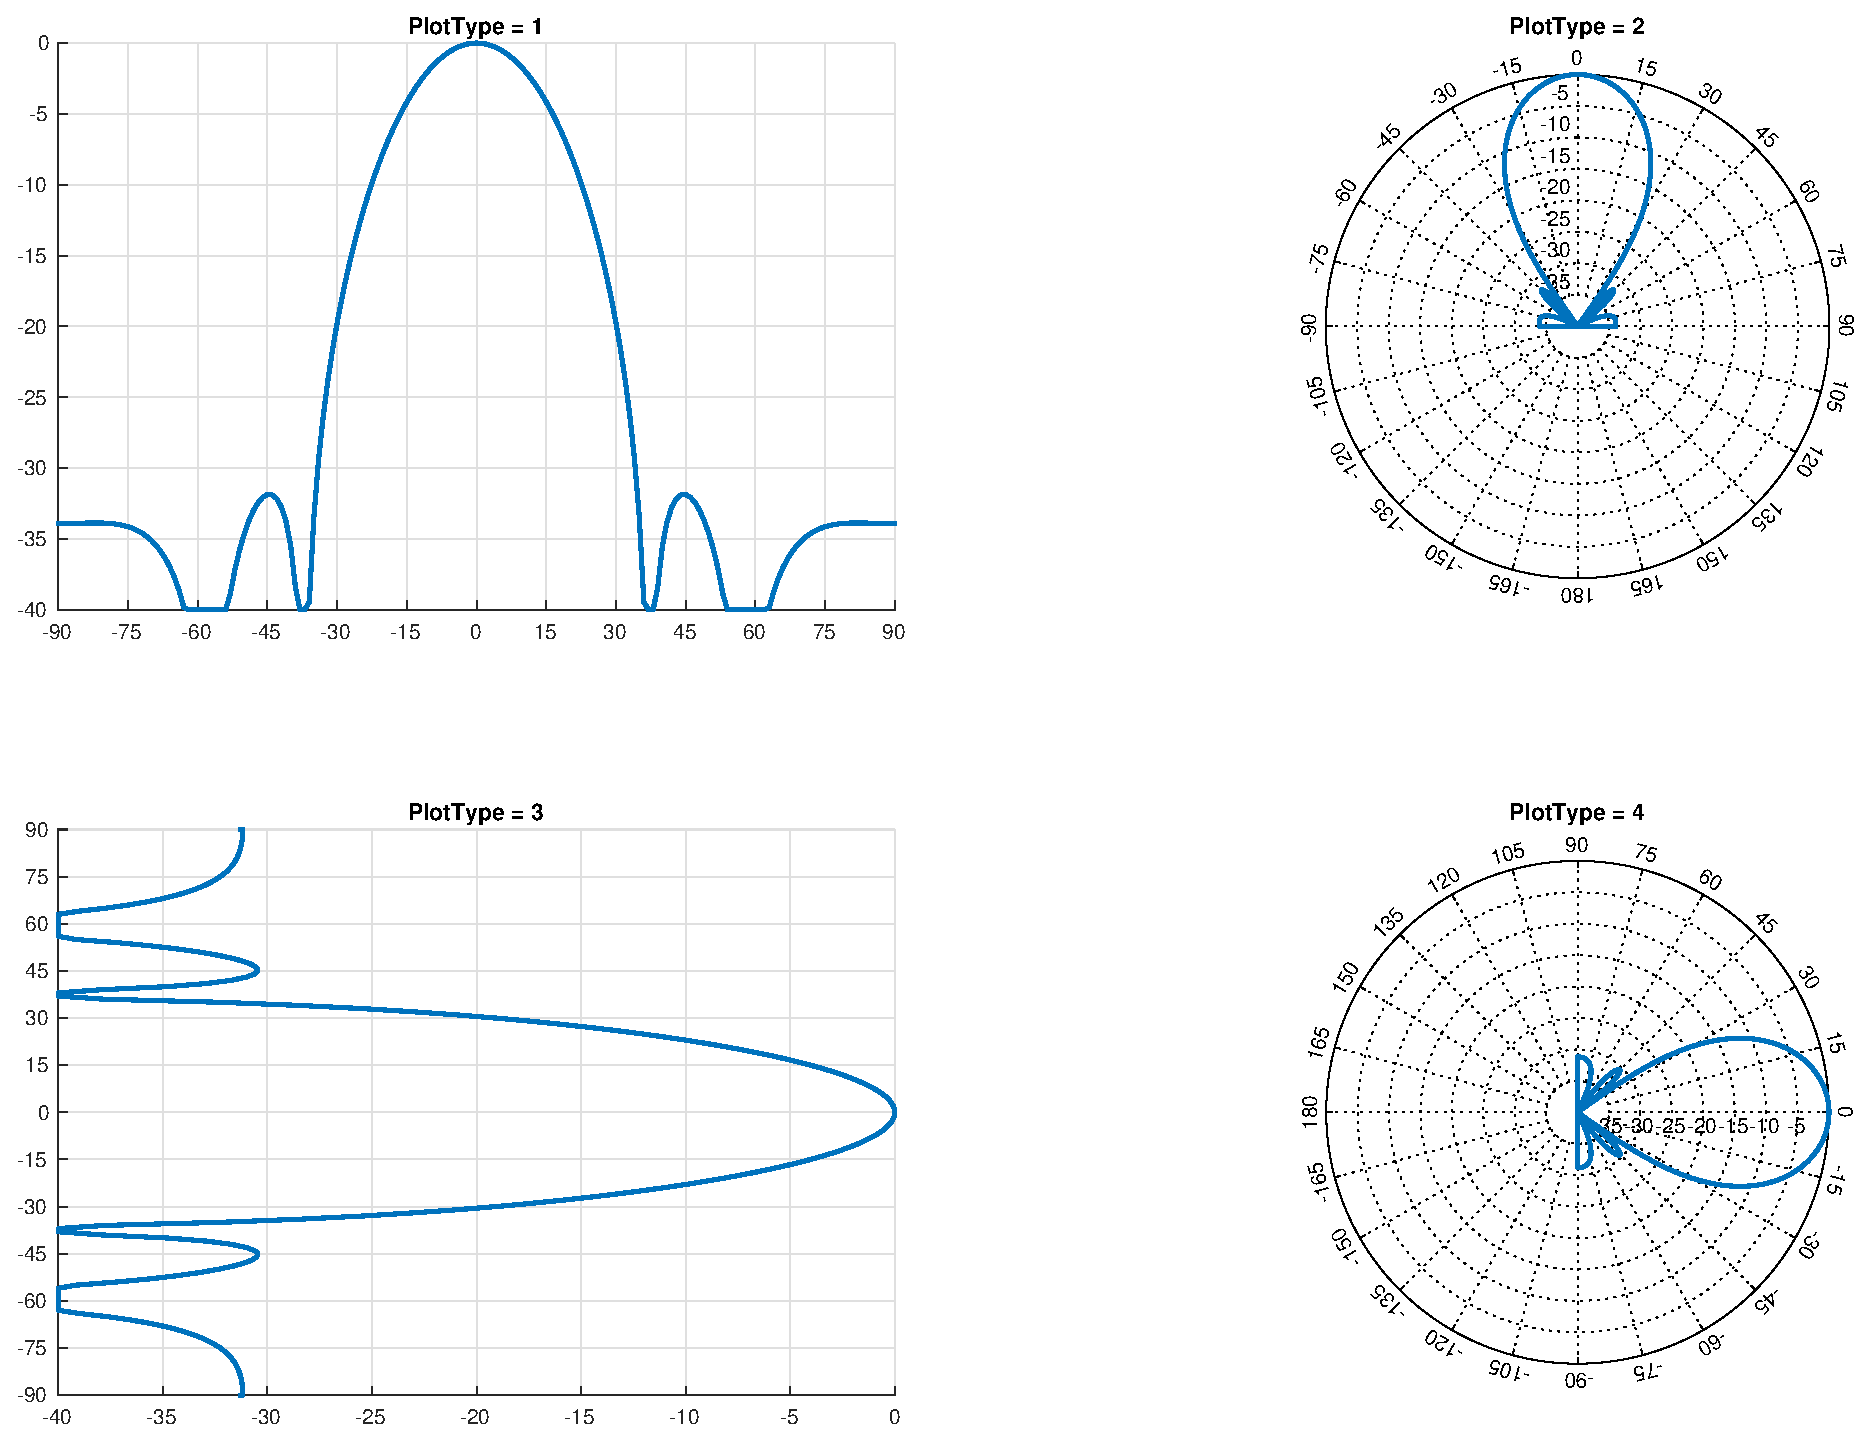
\includegraphics[width=7.75in]{Plot2DBPexamples}
\caption{\label{fig:Plot2DBPexamples}Example slices through rectangular planar array beam pattern}
\end{center}
\end{sidewaysfigure}

\clearpage
\section{Plotting 3D beam patterns}

The function \texttt{Plot3DBP.m} plots the three dimensional beam magnitude with decibel scaling. Usage instructions are shown in Listing~\ref{lst:Plot3DBP}. The three required inputs are elevation and azimuthal angle vectors, $\theta$ and $\psi$ in degrees, and the beam pattern matrix. 

The first optional input, \texttt{PlotType}, selects a plot with the beam pattern surface and color proportional to magnitude when its value is 1, and it selects a pot with the beam pattern color proportional to magnitude but drawn on a surface of constant radius when its value is 2. Examples of these two options are shown in the left and right panels of \figname~\ref{fig:SampleBeam} Those plots are for the example element, array, and beam defined in Listings~\ref{lst:SampleElement}, \ref{lst:SampleArray}, and \ref{lst:SampleBeam}.

The second optional input, \texttt{dBScale}, is a two-element vector with the minimum and maximum magnitudes in dB. The default values are -40 and 0 dB. It is common to use 0 dB for the maximum value, since the beam pattern is normalized by default.

The third optional input is the axis handle, \texttt{hax}, in which to plot the beam. This input has the same functionality as it does in \texttt{PlotArray.m}, and it allows the beam to be plotted with the array on the same axis. Matlab function \texttt{gca} can be used to specify the current axis.

The final optional inputs allow the beam to be offset according to the array position in the body frame. 

\lstinputlisting[firstline=2,lastline=26,caption={\texttt{Plot3DBP.m}},label={lst:Plot3DBP}]{../../mdl/Plot3DBP.m}

\clearpage
\begin{sidewaysfigure}[!ht]
\begin{center}
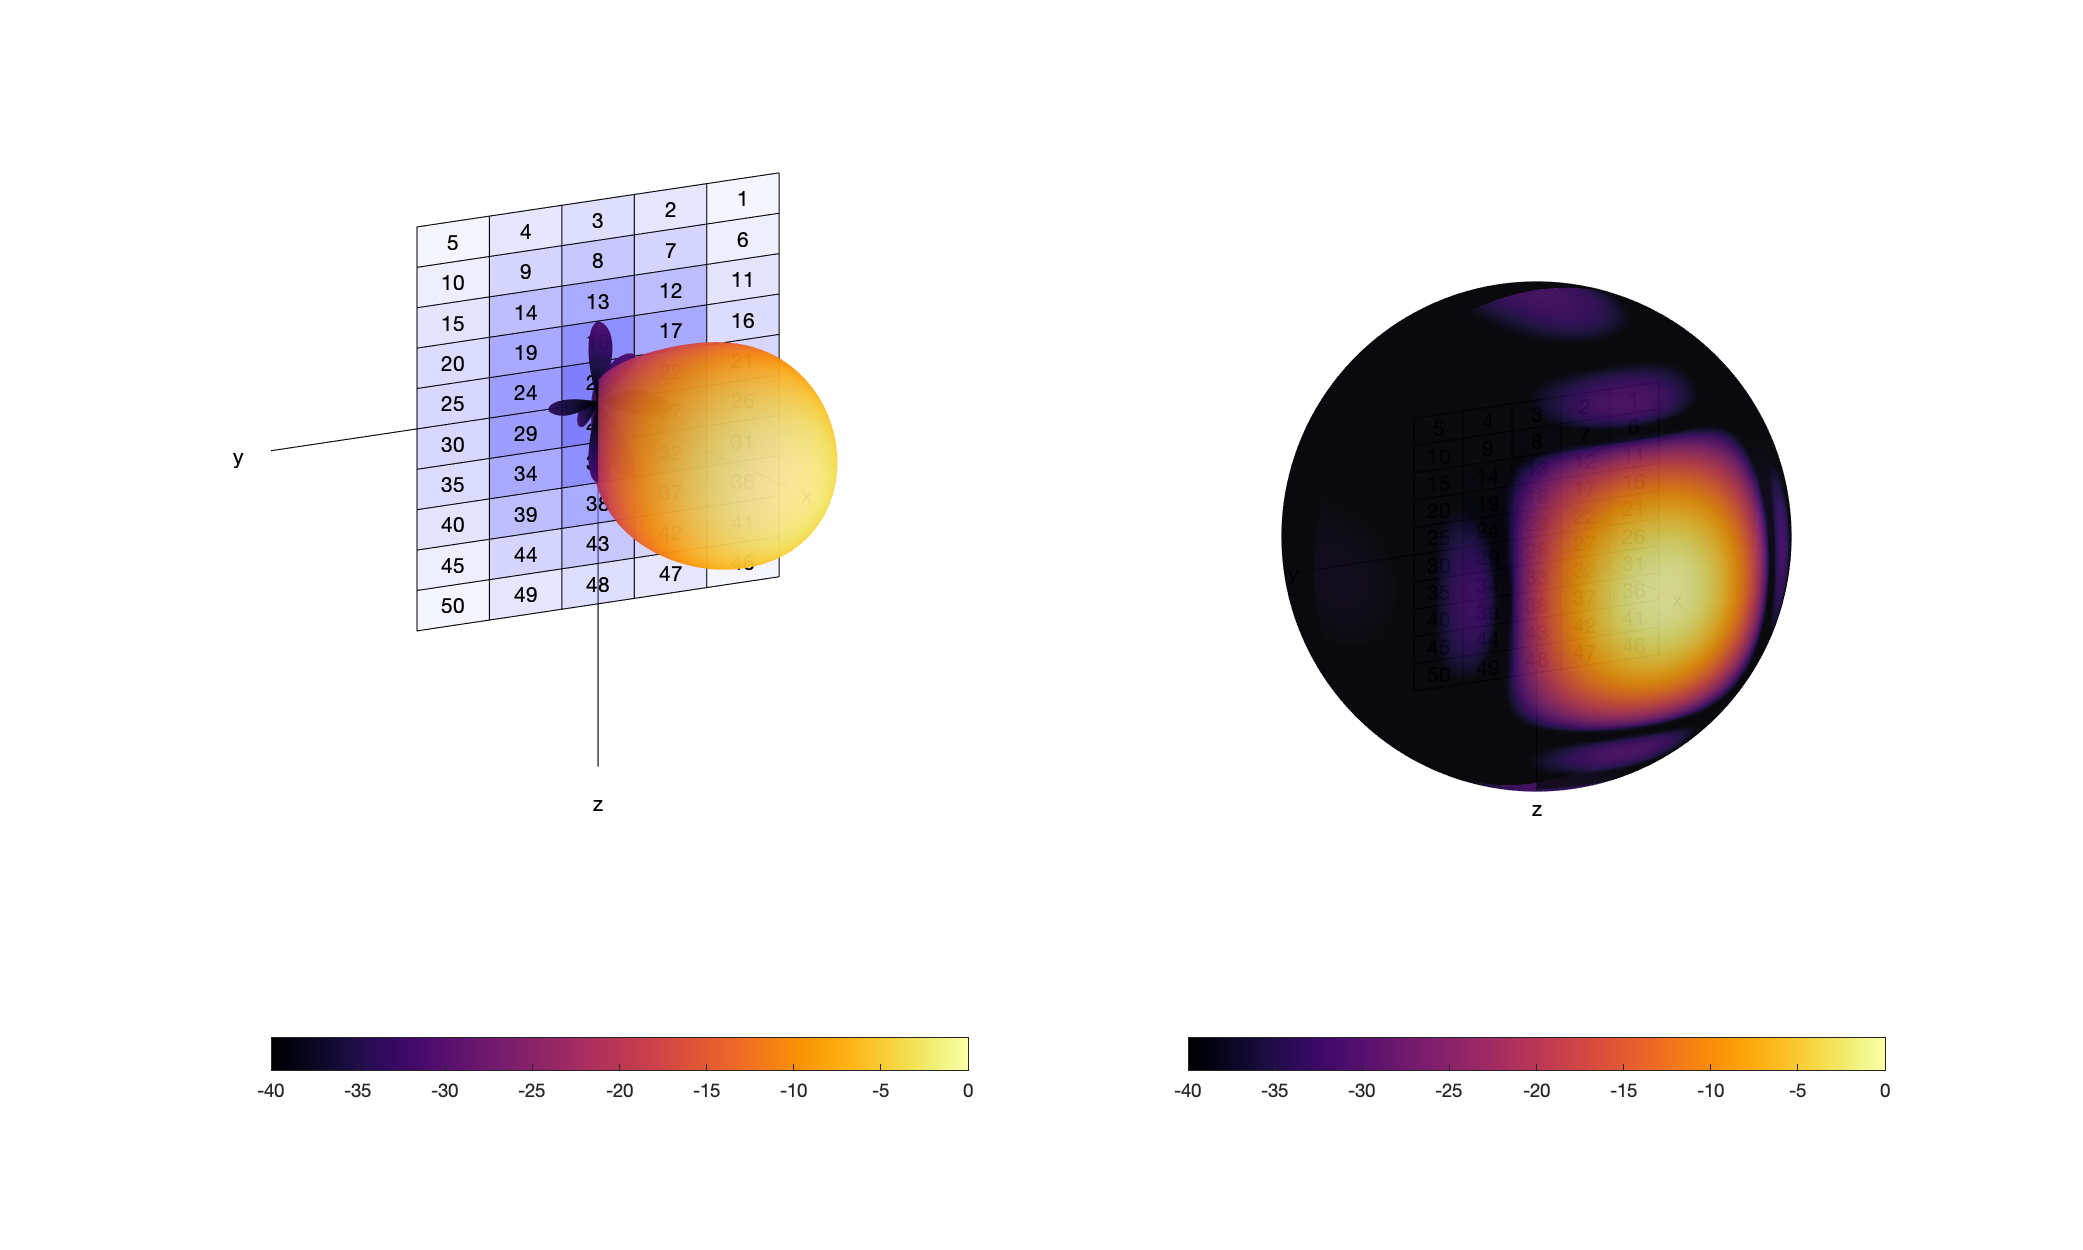
\includegraphics[width=7.75in]{SampleBeam}
\caption{\label{fig:SampleBeam}Example beam pattern for rectangular planar array}
\end{center}
\end{sidewaysfigure}

\clearpage
\section{Calculating beam width}

Beam width is the angular span over which the beam magnitude is within 3 dB of its peak value. Sonar Workbench contains two functions to calculate beam width: \texttt{BeamWidth.m} for 2D beams, which computes beam width in a single plane, and \texttt{BeamWidth3D.m} for 3D beams, which computes vertical and horizontal beam widths. Usage is shown in Listings~\ref{lst:BeamWidth} and \ref{lst:BeamWidth3D}.

\lstinputlisting[firstline=2,lastline=21,caption={\texttt{BeamWidth.m}},label={lst:BeamWidth}]{../../mdl/BeamWidth.m}

\lstinputlisting[firstline=2,lastline=26,caption={\texttt{BeamWidth3D.m}},label={lst:BeamWidth3D}]{../../mdl/BeamWidth3D.m}

There are two required parameters for \texttt{BeamWidth.m}. The first, \texttt{ang}, is a vector of angles in degrees over which the beam pattern slice is defined, and the second, \texttt{bp}, is the beam pattern at those angles, in linear units. The user can assist the function in locating the correct peak value to search around by specifying an approximate peak angle in the first optional parameter, \texttt{ang0}. The final optional parameter, \texttt{renorm}, instructs the function to re-normalize the beam pattern to have a peak magnitude of 0 dB before searching for the -3 dB angles. This can be useful for a steered beam whose peak magnitude is less than 0 dB. 

The output, \texttt{BW}, is the measured beam width in degrees. The function attempts to interpolate between input grid angles using spline interpolation of the beam magnitude in dB. The user can get a more precise measurement by using finer angle sampling. If \texttt{BeamWidth.m} can not calculate a valid beam width, it returns \texttt{NaN}.

\texttt{BeamWidth3D} has similar usage but with expanded support for an additional dimension. Its first three parameters are required, and correspond to angle vectors $\theta$ and $\psi$ in degrees and beam pattern matrix \texttt{BP} in linear units. The first two optional parameters, \texttt{theta0} and \texttt{psi0} serve the same purpose as \texttt{ang0} in \texttt{BeamWidth.m} for the elevation and azimuthal angles, respectively. The final optional parameter, \texttt{renorm}, is identical to that parameter in \texttt{BeamWidth.m}. There are two outputs, \texttt{BWV} and \texttt{BWH}, which are the vertical and horizontal beam widths in degrees, respectively. For the example beam in \figname~\ref{fig:SampleBeam}, the vertical and horizontal beam widths are calculated to be 26$^\circ$ and 25.6$^\circ$.

\section{Calculating directivity index}

Directivity Index (DI) is a measure of a beam's ability to filter spatially isotropic noise. It is the ratio of the noise level received by an omnidirectional sensor to the noise level received by the beam, expressed in dB. It is calculated from the Directivity (D) according to
\begin{equation}
DI(\lambda) = 10\log_{10}D(\lambda),\label{eq:DirectivityIndex}
\end{equation}
where
\begin{equation}
D(\lambda) = \frac{4\pi}{\int_0^{\pi}\int_0^{2\pi}|BP(\lambda,\theta,\psi)|^2d\psi{d\theta}}.\label{eq:Directivity}
\end{equation}

\texttt{CalculateDI.m} implements \eqnnames~(\ref{eq:DirectivityIndex}) and (\ref{eq:Directivity}) using numerical integration over a realized beam pattern. Usage is shown in Listing~\ref{lst:CalculateDI}.

There are three required parameters. The first two are angle vectors $\theta$ and $\psi$ in degrees, and the third is the beam pattern matrix \texttt{BP} in linear units. For best results, $\theta$ should span 180$^\circ$ vertically, and $\psi$ should span 360$^\circ$ horizontally. If instead, the beam pattern is defined as a subset of these angles, \texttt{CalculateDI.m} assumes the beam pattern value is exactly zero outside the defined region. There is a single output, \texttt{DI}, which is the directivity index in dB.

\lstinputlisting[firstline=2,lastline=18,caption={\texttt{CalculateDI.m}},label={lst:CalculateDI}]{../../mdl/CalculateDI.m}

\newpage
\bibliographystyle{ieeetr}
\bibliography{SonarWorkbench}

\end{document}
